\section{Branching}

\begin{frame}[t]
  \frametitle{Outline}
  \framesubtitle{Why? and little bit of How?}
  \tableofcontents[currentsection,hideallsubsections] 
\end{frame}

\begin{frame}[t]{What will be covered in this section?}
  \begin{itemize}
    \item Why Branching?
    \item How to Branch.
    \item[]
    \item Read Chapter 3 of {\it Pro Git} for more information.
    \item[]
    \item Branching and merging are fundamental to the use of Git.  
      \begin{itemize}
        \item In other VC software system branching and merging are either
          imposible or very, very difficult.
        \item Git makes it easy!
      \end{itemize}

    \item I'm hoping to have time to talk about this, but I expect to have run
      out of time.  It's okay, working on just the master branch for now is a
      good starting place.  Learn all the verbs needed to work on one branch and
      then the details to learn branching will come as a natural next step.
  \end{itemize}
\end{frame}

\begin{frame}[t]
  \frametitle{Why is Branch?}
  \begin{itemize}
    \item Develpment off of the master branch.
    \item Work in a sandbox for features.
    \item What's down this rabit hole?
    \item[]
    \item ``I've got this great idea!  Wait, \#$@$!!?\%, it's not going
      anywhere.  Well, maybe?  I'd done know.'' $\leftarrow$ Make a branch! :)
  \end{itemize}
\end{frame}

\begin{frame}[t]{}
  \frametitle{Branching Model}
  \framesubtitle{ \url{http://nvie.com/posts/a-successful-git-branching-model/} }

  \begin{center} 
    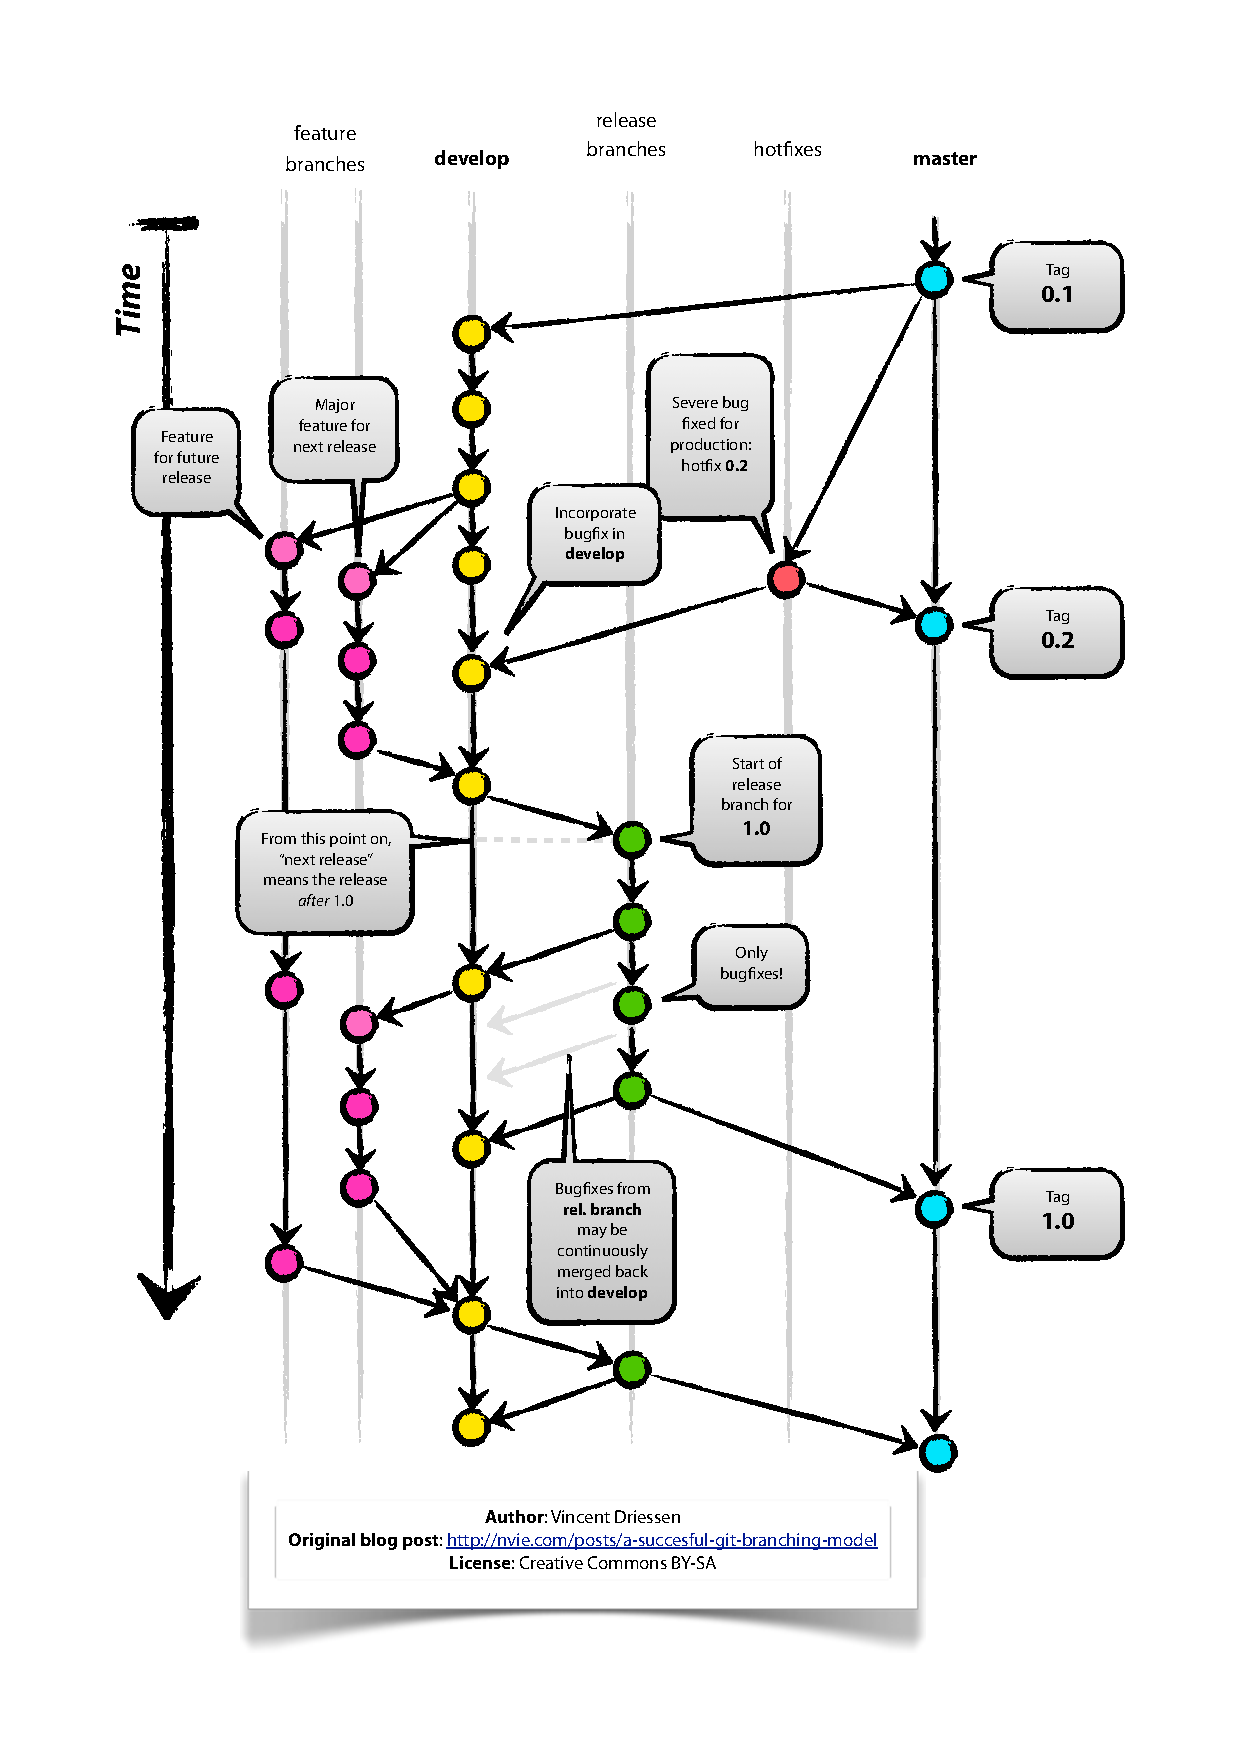
\includegraphics[height=2.75in]{./images/Git-branching-model}
  \end{center}
\end{frame}


% \subsection{Branches in a Nutshell}
% \begin{frame}[t]{}
% \end{frame}
% 
% \subsection{Basic Branching and Merging}
% \begin{frame}[t]{}
% \end{frame}
% 
% \subsection{Branch Management}
% \begin{frame}[t]{}
% \end{frame}
% 
% \subsection{Branching Workflows}
% \begin{frame}[t]{}
% \end{frame}
% 
% \subsection{Remote Branches}
% \begin{frame}[t]{}
% \end{frame}
% 
% \subsection{Rebasing}
% \begin{frame}[t]{}
% \end{frame}
% 
% \begin{frame}[t]{}
% \end{frame}
% 
% 
